\section{The Evolution of Systems Thinking}\index{The Evolution of Systems Thinking}

Systems thinking is subjective. It is the cognitive and cognation process of seeking understanding about the interactive influences of entities within a whole. Thinking about the engineering of systems, as presented here, encompasses entities and wholes within the context of our existence.

But systems thinking is not pervasive enough, nor is it adequately comprehensive. 

\begin{enumerate}
\item The boundary of a system is a decision made by an observer, or a group of observers.
\item A system can be nested inside another system.
\item A system can overlap with another system.
\item A system is bounded in time.
\item A system is bounded in space, though the parts are not necessarily co-located.
\item A system receives input from, and sends output into, the wider environment.
\item Science systems thinkers consider that:
\item A system is a dynamic and complex whole, interacting with a structured functional unit. Energy, material, and information flow among the different elements that compose the system;
\item A system is a community situated within an environment. Energy, material, and information flow from and to the surrounding environment via semi-permeable membranes or boundaries;
\item Systems are often composed of entities seeking equilibrium but can exhibit oscillating, chaotic, or exponential behavior.
\end{enumerate}

A holistic system is any set (group) of interdependent or temporally interacting parts. Parts are generally systems themselves and are composed of other parts, just as systems are generally parts or halons of other systems.

Two parts to be considered: 1) the desired human-made system and, 2) the engineering of that system. Both are within the goal of focused systems thinking on the well-being of humans that exist within the human-modified world; that is, the world emerging from the natural world through purposeful design by humans.

\subsection{World Focused Systems Thinking}\index{World Focused Systems Thinking}

World focused systems thinking starts with the premise that “systems science” exists, or at least a “theory of systems” is available to define systems and system properties. These properties of a system – which can be either natural or human-made, and which can exhibit a greater or lesser degree of adaptive behavior – are independent of how and why it was created. The nature of such systems is independent of human intentionality, and we see similar or identical system properties and patterns recurring across different domains of application.

Systems thinking is the process of understanding how things influence one another within a whole. In nature, systems thinking examples include ecosystems in which various elements such as air, water, movement, plants, and animals work together to survive or perish. In organizations, systems consist of people, structures, and processes that work together to make an organization healthy or unhealthy. In economics …

World focused systems thinking seems to be a stretch. But, it is necessary as the basis for looking beyond the world in which we live. This is for completeness within the scope of what is known by humans currently.

Consider Figure 1.2. Depicted is a view beyond the world in which we live. This is deemed necessary to acknowledge the universe of which our world is a part. We know little about that universe and others being mentioned. And, there is no attempt in this book to reach that far in bringing the human-made into being. Maybe someday!

\begin{figure}[h]
\centering
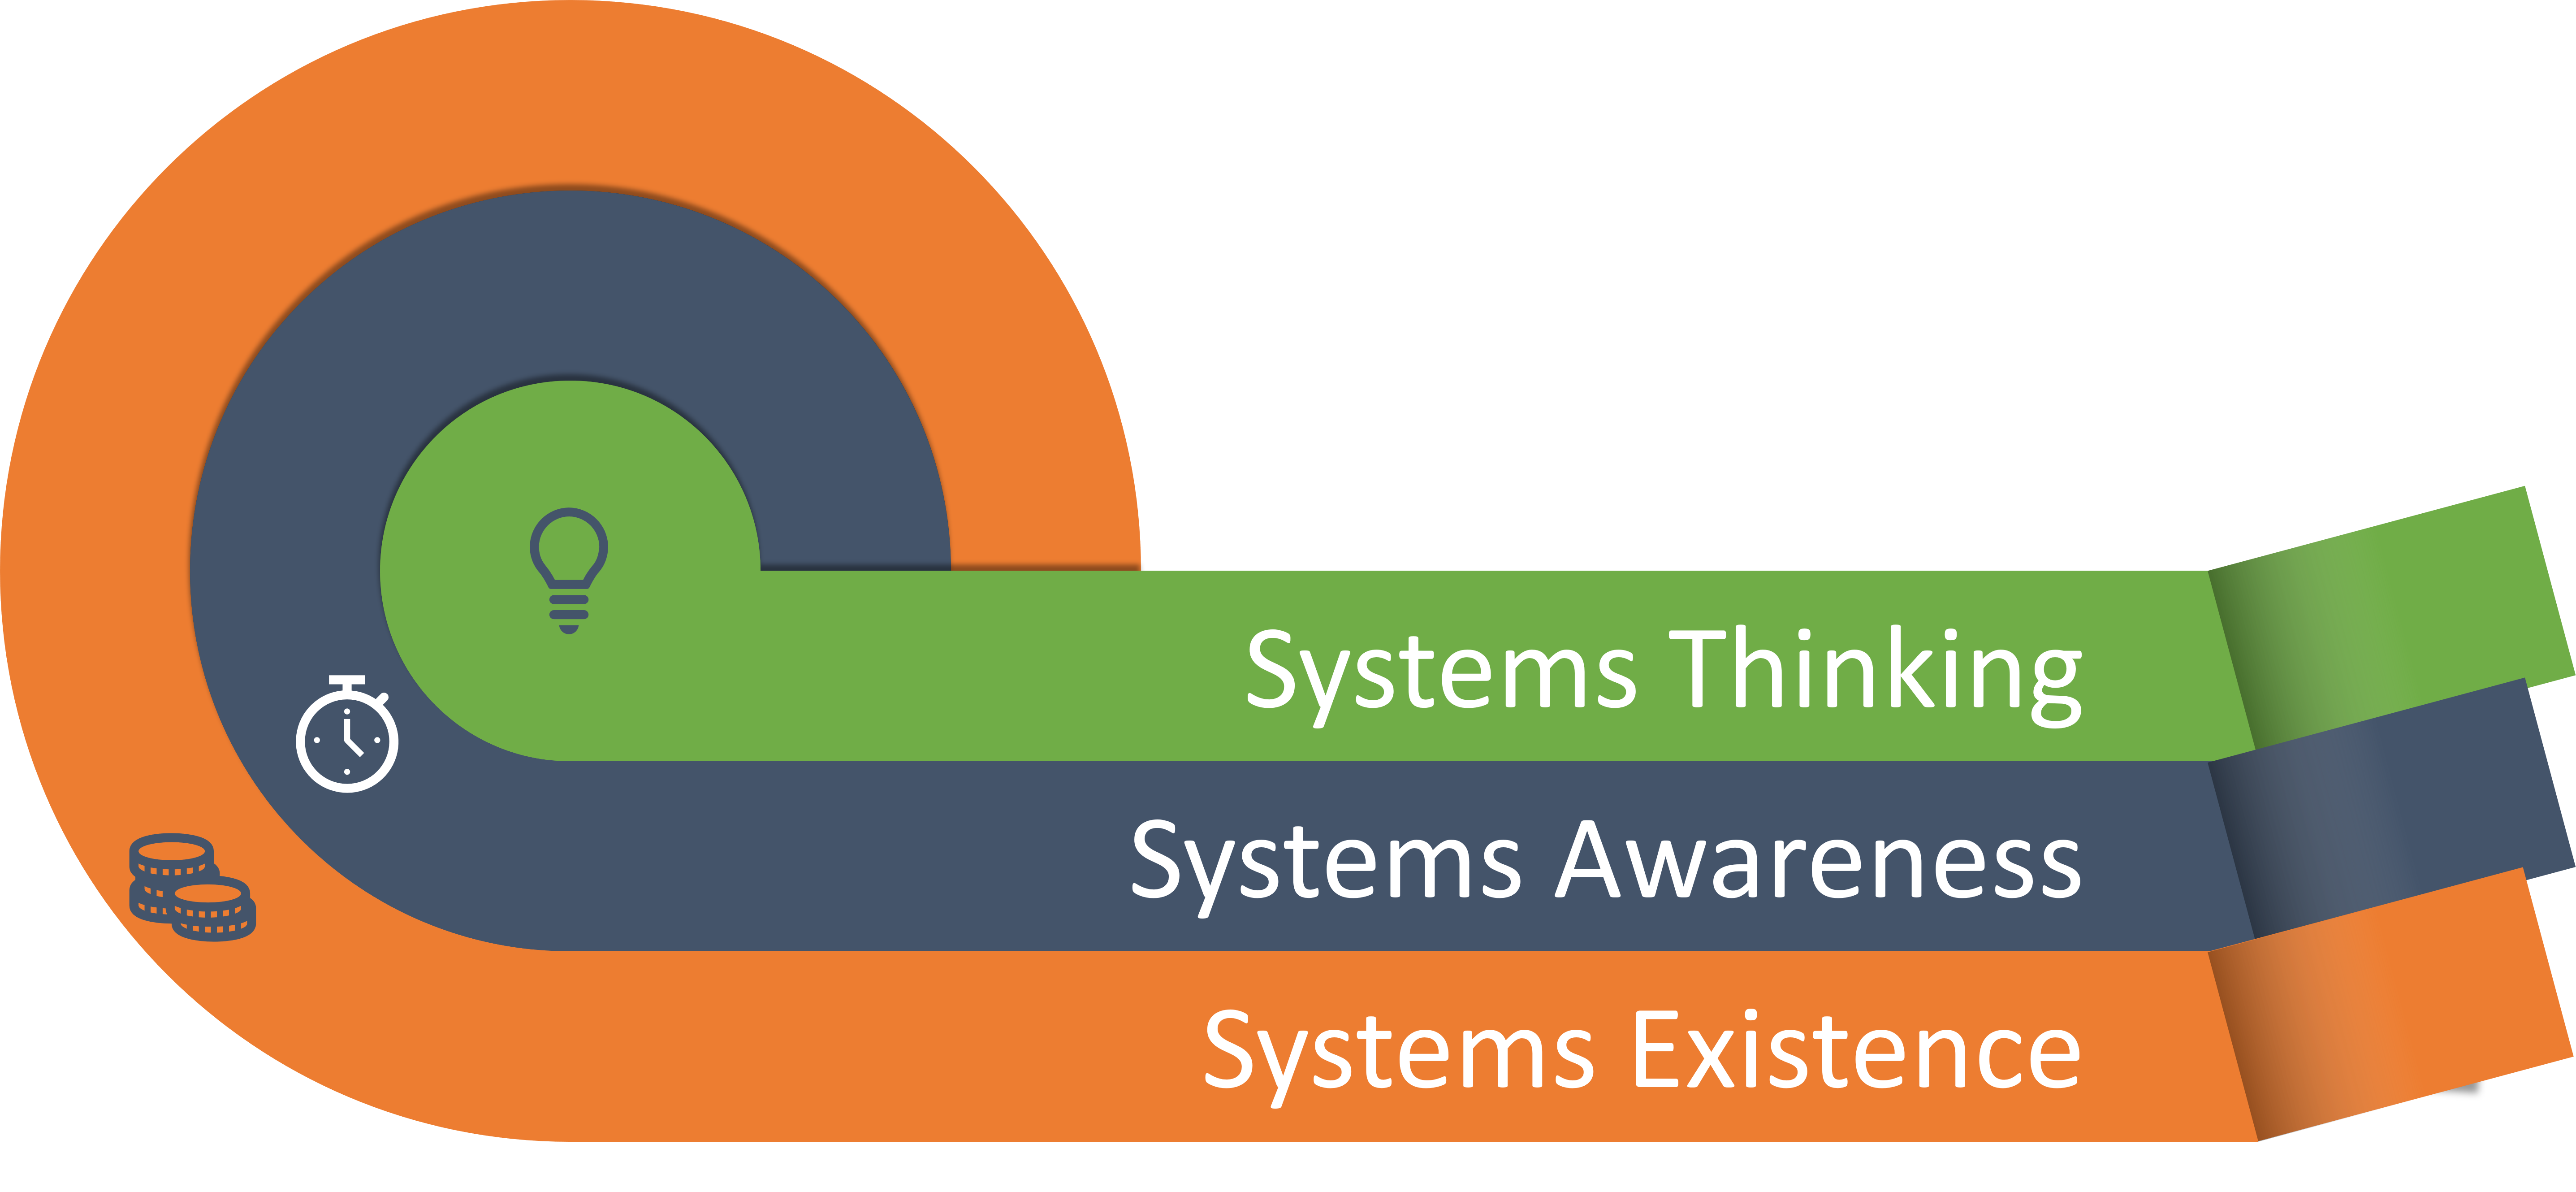
\includegraphics[width=0.9\textwidth]{systemsThinkingSnail.png}
\caption{Complete experimental setup (left) with close-up view of stage (right).}
\label{fig:systemsThinkingSnail}
\end{figure}

Figure 1.2 is conceptual in nature and self-explanatory. In science, it is argued that the only way to fully understand why a problem or element occurs and persists is to understand the parts in relation to the whole. [3] Standing in contrast to Descartes’s scientific reductionism and philosophical analysis, it proposes to view systems in a holistic manner. Consistent with systems philosophy, systems thinking concerns an understanding of a system by examining the linkages and interactions between the elements that compose the entirety of the system.

Science systems thinking attempts to illustrate that events are separated by distance and time and that small catalytic events can cause large changes in complex systems. Acknowledging that an improvement in one area of a system can adversely affect another area of the system, it promotes organizational communication at all levels to avoid the silo effect. Systems thinking techniques may be used to study any kind of system – natural, scientific, engineered, human or conceptual.

Systems thinking has been defined as an approach to problem solving, by viewing “problems” as parts of an overall system, rather than reacting to specific part, outcomes or events and potentially contributing to further development of unintended consequences. Systems thinking is not one thing but a set of habits or practices within a framework that is based on the belief that the component parts of a system can best be understood in the context of relationship with each other and with other systems, rather than in the isolation. Systems thinking focuses on cyclical rather than linear cause and effect.

\subsection{Think Globally, Act Locally}\index{Think Globally, Act Locally}

The approach adopted in this book is to recommend to globally conscious people and youth (especially STEM participants) to acquire an interest in the degree to which human designs act to modify the natural world.
\begin{enumerate}
\item More attention to design can alleviate problems revealed during operations because operational outcomes are inherent and linked to the physics of design
\item The on-line linking of individual designer’s decisions to evaluation at the system level and to stakeholder value is becoming more technically feasible. How?
\end{enumerate}

Define the system design space and partition it into the Functional domain, the Design Dependent Parameter domain, and the Optimization domain, etc.
Design Dependent Parameters (DDP’s) are suggested as the most overarching and most LINK between human designers and the human modified world. They established the design space and specific predicted and/or estimated values thereof drive design evaluation.
Design evaluation is the compass for stumbling through the design space in search of a modified world judged to be satisfactory by stakeholders.

	Add material by Kathia Laslo, PhD who directs Staybook University’s program in Leadership of Sustainable Systems . . . 
    
\subsection{Think About the End Before Beginning}\index{Think About the End Before Beginning}

From the thinking of Leonardo da Vinci
\begin{itemize}
\item WHY “To Make the World Better for People” (Retitle source here)
\item Human-made entities should be designed to satisfy human needs, wants, and objectives effectively, while minimizing system life-cycle cost as well as the intangible costs of ecological and societal impacts on the natural world
\item HOW ``Adopt and Practice Systems Thinking and Engineering''
\item A technologically based interdisciplinary process for bringing systems, products, structures, and services (human-made entities) into being
\end{itemize}

Reorient the Organization: Organization, humankind’s most important innovation, is the time-tested means for bringing human-made entities into being. While the main focus is nominally on the entities themselves, Systems Engineering embraces better strategy. Systems Engineering concentrates on what the entities do before determining what the entities are, with form following function. That is, instead of offering systems or system elements and products per se, the organizational focus should shift to designing, delivering, and sustaining functionality, a capability, or a solution.